\chapter{Experimento II: medición indirecta usando un circuito resonante}

% recuerda incluir que las referencias GuiaLAB-MIT y GuiaLab-SUNY son guias de laboratorio donde se explican este experimento con circuito resonante

%recuerda incluir porque en la suma de las densidades que dice la HCC en este caso importa poco la componente electromagnetica y no es una mala aproximación solo tratar con la parte gravitacional (secreto: esta ultima es muchos ordenes de magnitud (ya eso lo calculó greaves en algun lado) mayor y ademas como el circuito es el mismo la parte electromagnetica más cercana se mantiene) 

AQUI VA EL RESUMEN DEL CAPITULO
\section{Fundamentos teóricos: Electrodinámica y Resonancia}


El objetivo de este planteamiento es el de utilizar la relación de la velocidad de la luz con la permitividad eléctrica $\varepsilon_0$ y la permeabilidad magnética $\mu_0$ dada por
\begin{equation} \label{permitividadyc}
c=\frac{1}{\sqrt{\varepsilon_0\,\mu_0}}
\end{equation}
Donde usaremos el hecho de que $\mu_0$ es una constante cuyo valor es $\mu_0 = 4\pi\cdot 10^{-7}$H/m, por lo que basta con medir la permitividad eléctrica con precisión.

Por otro lado, la capacitancia de un capacitor de placas paralelas está dada por
\begin{equation} \label{capacitanciaplacasparalelas}
C_a=\varepsilon_0\,\frac{A_c}{d}=\frac{1}{c^{2}\mu_0}\,\frac{A_c}{d}
\end{equation}
Con $A_c$ siendo el área de las placas y $d$ la separación entre ellas. En cualquier capacitor se cumple que su capacitancia depende de su geometría y del material, con ecuaciones análogas a \ref{capacitanciaplacasparalelas} en cada caso. Entonces, medir la capacitancia de un capacitor permite conocer el valor de $\epsilon_0$ que es equivalente a medir la velocidad de la luz. 

Una manera de medir indirectamente la capacitancia $C$ es conectar dicho capacitor en serie (o en paralelo) con una resistencia $R$ y un inductor $L$ para crear un circuito R-L-C. La característica principal de este tipo de circuitos es que la energía almacenada en el capacitor se va liberando y a su vez almacenando en el inductor, para ser luego este último el que proporcione la energía al capacitor, en este proceso la corriente eléctrica cambia su dirección de modo que la corriente es alterna. Al aplicarle una corriente de frecuencia $f$ al circuito este responde con la producción de una corriente con la misma frecuencia y distinta amplitud, la amplitud de la corriente será máxima cuando la frecuencia aplicada sea igual a la frecuencia de resonancia del circuito la cual está dada por

\begin{equation} \label{frecuenciaResonancia}
f_0=\frac{1}{2\pi\sqrt{LC}}
\end{equation}

Aquí $L$ es la inductancia de la bobina, entonces si consideramos un solenoide toroidal con núcleo vacío de $N$ vueltas, con área transversal $A_L$ y radio $r$ la inductancia está dada por

\begin{equation}
L=\frac{\mu_0\,N^{2}\,A_L}{2\pi r}
\end{equation}

Como el fin último es medir la velocidad de la luz en diferentes puntos geográficos, si se usa el mismo inductor en el circuito el $L$ no se verá modificado y lo tomamos como una constante. Así al hacer la sustitución de ecuación \ref{capacitanciaplacasparalelas} en \ref{frecuenciaResonancia} nos queda
\begin{equation}
f_0=\frac{c}{2\pi\sqrt{\dfrac{L\,A_c}{d\,\mu_0}}}=k_0\,c
\end{equation}
Donde $k_0$ sería una constante dada por
\begin{equation}
k_0=\frac{1}{2\pi\sqrt{\dfrac{L\,A_c}{d\,\mu_0}}}
\end{equation}
Los valores esperados de $c$ según la hipótesis de Cespedes-Curé para cada uno de los puntos donde se realizarán mediciones ya se expusieron previamente en la tabla \ref{tab:Valores_c_esperados}. Para calcular los cambios esperados en la frecuencia de resonancia del mismo circuito pero en estas tres locaciones tomemos el valor de la constante como $k_0=0.002165397~\text{m}^{-1}$, este cálculo se hace con los siguientes datos $L=6.70\times 10^{-3}\,\text{H}$, $A_c=0.04\,\text{m}^{2}$, $d=0.001\,\text{m}$ y $\mu_0=4\pi\cdot 10^{-7} $ H/m.

\begin{table}[h!]
\centering
\begin{tabular}{lccc}
\toprule
Localidad & Velocidad $C$ m/s & $f_0$ Hz & $f_0/f_{\text{Carmen de Urea}}$\\
\midrule
Carmen de Urea & 299792471.69 & 103318.57\textcolor{red}{0664} & 1\\
USB            & 299792473.97 & 103318.57\textcolor{red}{1449} & 1.000000008\\
Teleférico     & 299792475.47 & 103318.57\textcolor{red}{1966} & 1.000000013\\
\bottomrule
\end{tabular}
\caption{Estimaciones de la frecuencia de resonancia de un circuito RLC según \ac{HCC} en las tres localidades planteadas.}
\end{table}

Se señalan en rojo las cifras que cambian en cada locación. Vemos que para este caso sería necesario alcanzar una resolución de micro Hz para poder apreciar el cambio.


\subsection{Factor de calidad Q}

Es importante señalar que para los circuitos resonantes existe un factor llamado calidad $Q$, el cual mide la eficiencia del circuito, es decir cuán bien el circuito almacena energía en comparación con la energía que pierde. Un alto valor de $Q$ implica una banda de frecuencia estrecha, como para un circuito RLC se tiene que
\begin{equation} \label{factorQ}
Q=\frac{\omega L}{R}
\end{equation}



Basta con disminuir la resistencia y aumentar la inductancia para asegurarnos de tener una función bien estrecha que permita obtener un valor bien preciso de la frecuencia de resonancia.

\begin{figure}[h!]
  \centering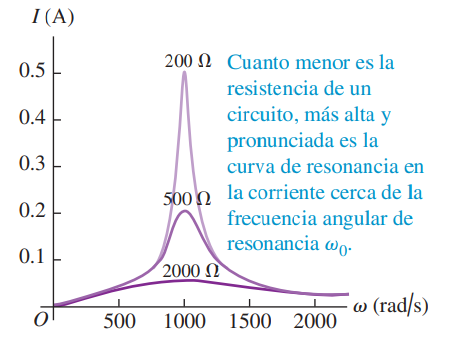
\includegraphics[width=0.6\linewidth]{FactorQ-zemansky.png}\caption{Comportamiento del factor Q según la resistencia en el circuito \cite{searsZemanskyV2}.}
\end{figure}

\section{Planteamiento del procedimiento experimental}

\begin{figure}[h!]\centering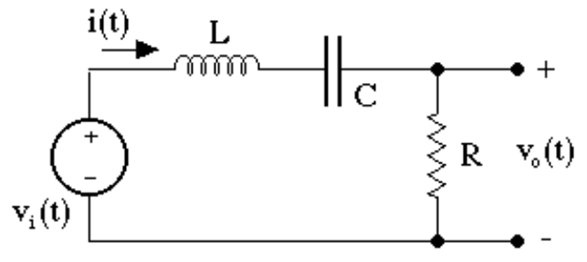
\includegraphics[width=0.5\linewidth]{SUNY-circuito.png}\caption{Circuito RLC en serie planteado por la referencia \cite{GuiaLab-SUNY}.} \label{fig:circuitoGUIASUNY}\end{figure}

Usar la relación \ref{permitividadyc} para estimar el valor de la velocidad de la luz no es algo nuevo \cite{GuiaLab-SUNY}\cite{GuiaLAB-MIT}. Tomemos como punto de partida el montaje experimental plantado en \cite{GuiaLab-SUNY}, donde se usa el esquema de la figura \ref{fig:circuitoGUIASUNY}. Ellos plantean determinar los valores de $L$ y $C$ a partir de las caracteristicas físicas de los componentes electronicos, sin embargo en nuestro caso eso no es necesario ya que el objetivo es comparar el comportamiento del circuito en las tres locaciones, y para ello basta con distinguir el pequeño corrimiento del pico en el barrido de frecuencia que predice la \ac{HCC}.

Un cambio adicional necesario en el montaje experimental es que el mismo se pueda conectar a una computadora, o un Arduino, que permita controlar tanto los cambios de frecuencia de la fuente variable como la amplitud de la corriente en el circuito simultáneamente y de manera automática, esto con el fin de realizar miles de mediciones en un periodo de tiempo corto y para trazar una gráfica exenta de errores humanos.

\subsection{Análisis de la respuesta en serie y simulaciones de sensibilidad}

Supongamos que trabajamos con los mismos valores con los que se calculó la frecuencia de resonancia antes, la amplitud de la corriente en el circuito está dada por
\begin{equation}
I=V/Z
\end{equation}
Donde $Z$ es la impedancia, por lo tanto
\begin{equation}
I=\frac{V}{\sqrt{R^{2}+\left(2\pi f L-\dfrac{1}{2\pi f C}\right)^{2}}}
\end{equation}
Al sustituir la ecuación (2) se tiene
\begin{equation}
I=\frac{V}{\sqrt{R^{2}+\left(2\pi f L-\dfrac{1}{2\pi f}\,\dfrac{c^{2}\mu_0\,d}{A_c}\right)^{2}}}
\end{equation}
Simplificando un poco
\begin{equation}
I=\frac{V}{\sqrt{R^{2}+\left(2\pi f L-\dfrac{2\,c^{2}\,d\cdot 10^{-7}}{f\,A_c}\right)^{2}}}
\end{equation}
A continuación, una gráfica de esta función usando valores de la frecuencia que van en pasos de $0.1\,\mu\text{Hz}$ (30\,000 puntos graficados en total), donde lo único que cambia es la velocidad de la luz $c$ según los valores que se predicen en la hipótesis de Cespedes-Cure, además el valor de la resistencia usado es de $0.0168\,\Omega$, que es equivalente a un cable de cobre de un metro de longitud y sección transversal de 1 mm$^{2}$, y para el voltaje se usó $1\,\text{mV}$.

\begin{figure}[h!]\centering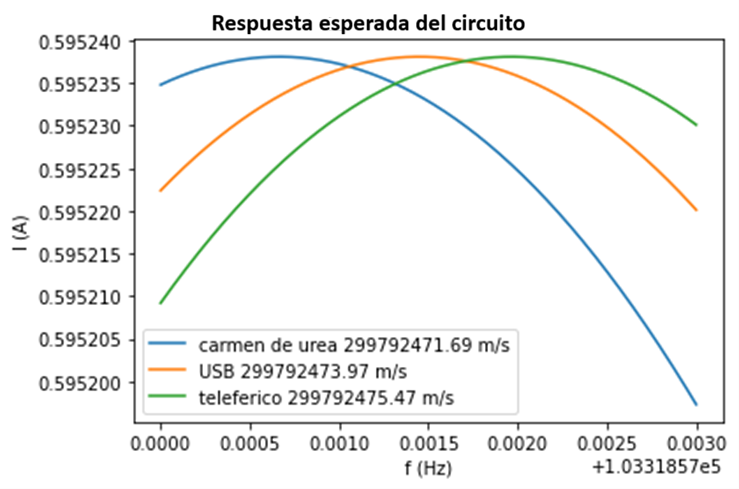
\includegraphics[width=0.90\linewidth]{Simulacion-respuesta1.png}\caption{Curvas $I(f)$ para las tres locaciones.}\label{fig:simulacion1}\end{figure}

En la figura \ref{fig:simulacion2} se puede ver cómo de estrecha es la gráfica en realidad, en este caso se graficaron 10000 puntos igualmente espaciados, ya que con eso es suficiente para darnos una idea de la forma de la función (11) en este caso donde el barrido es entre 103315 Hz y 103322 Hz.

\begin{figure}[h!]\centering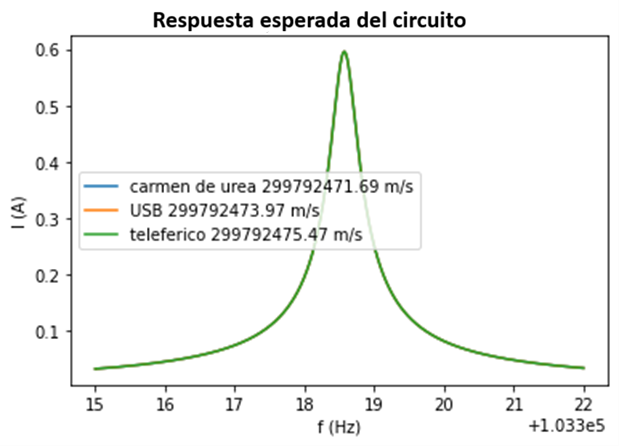
\includegraphics[width=0.90\linewidth]{Simulacion-respuesta2.png}\caption{Detalle de la curva $I(f)$.}\label{fig:simulacion2}\end{figure}

Para que las tres curvas correspondientes a las tres locaciones se puedan identificar correctamente es necesario medir la amplitud de corriente con gran presicion. Si consideramos un multímetro comercial muy preciso conectado en serie dentro del circuito resonante tenemos un problema: las apreciaciones para estos rangos de frecuencias son muy grandes. Es por esto que se obtó por trabajar midiendo la respuesta del voltaje en lugar de la corriente.

%Por ejemplo, para el multímetro más preciso que encontré [4] el rango de 1 A sería perfecto para los valores con los que se está trabajando ya que el error asociado es del orden de 1 $\mu$A, sin embargo, la frecuencia máxima a la que puede realizar mediciones de corriente es 10\,kHz. Disminuir tanto la frecuencia de resonancia de nuestro circuito no es una opción, ya que implica que los cambios en el valor de la frecuencia debido a un cambio en la velocidad de la luz no podrían alcanzarse con la fuente de corriente alterna. Recordemos que dependemos de que la fuente pueda variar con ``pasos'' lo suficientemente pequeños como para alcanzar la frecuencia de resonancia exacta (o por lo menos muy cercana) del circuito en cada uno de los puntos geográficos donde se medirá. Entramos entonces en un ciclo: necesitamos una frecuencia alta para poder medir los cambios de ella (eje $x$ de la gráfica) y necesitamos medir con precisión la corriente (eje $y$) para lo cual se necesita disminuir al menos en dos órdenes de magnitud la frecuencia.Una alternativa pudiera ser el uso de un osciloscopio conectado como lo indica la referencia [2], actualmente estoy trabajando en esa posibilidad\ldots

  


\subsection{Alternativa de medición: Configuración en paralelo}

Otra forma de realizar el circuito es mediante una conexión en paralelo del capacitor y el inductor, como se ve en la figura \ref{fig:RLCparalelosencillo}.

\begin{figure}[h]\centering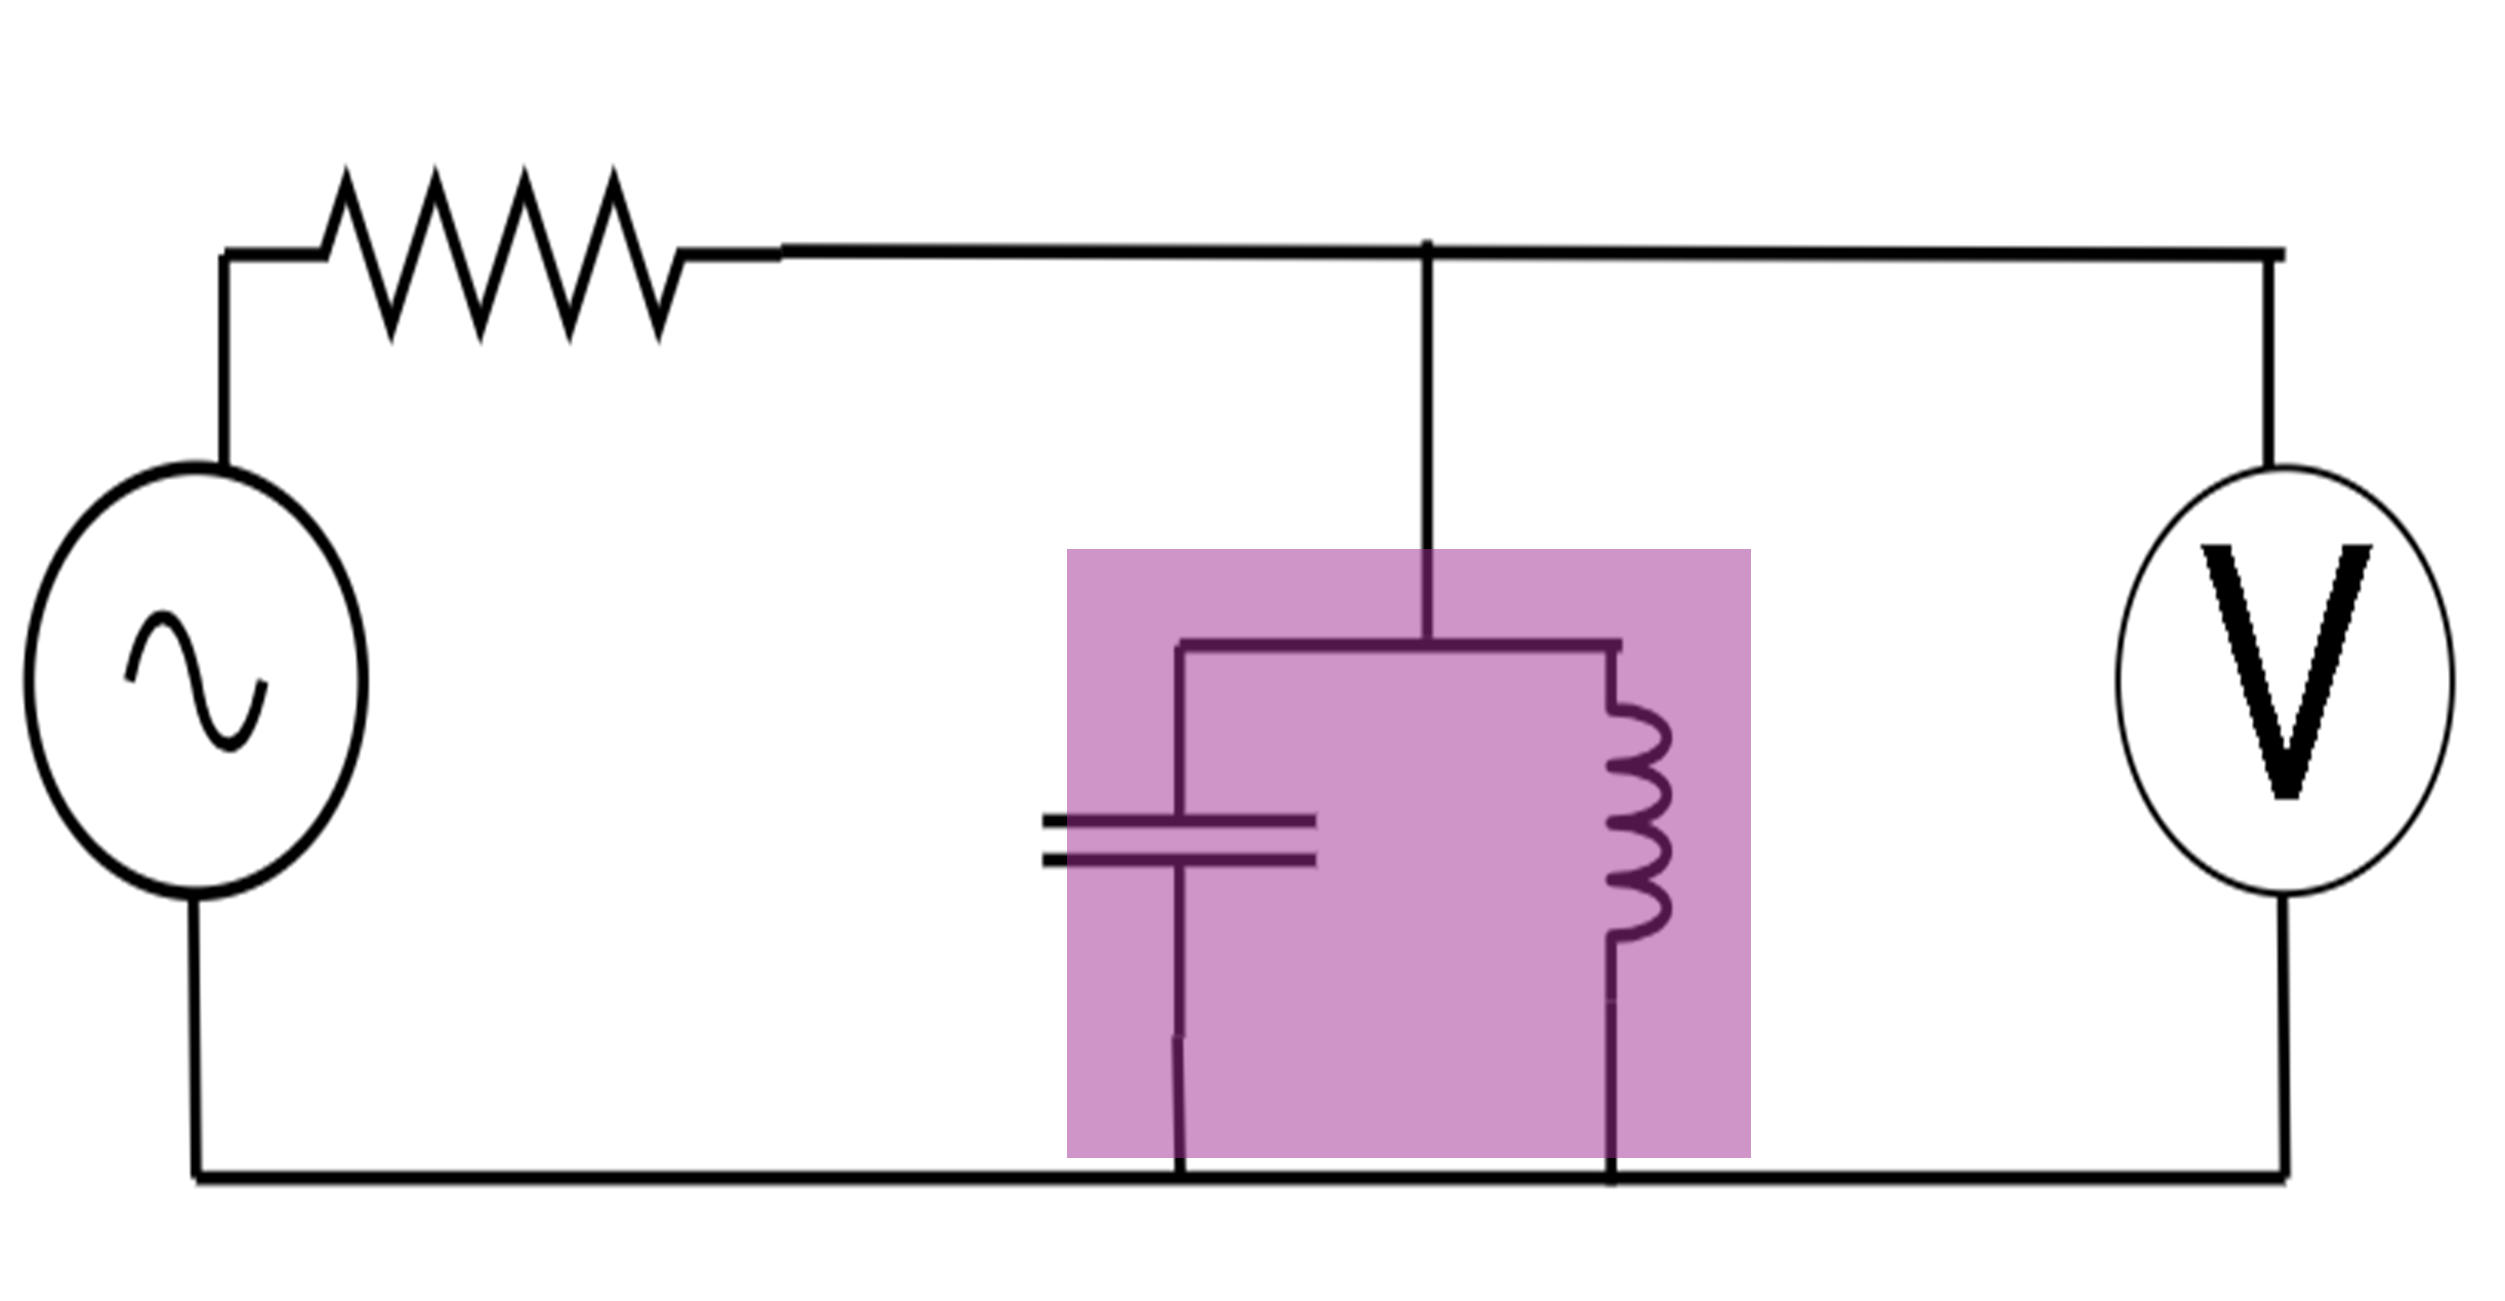
\includegraphics[width=0.45\linewidth]{CL-paralelo-sencillo.png}\caption{Esquema básico de circuito RLC en paralelo.} \label{fig:RLCparalelosencillo}\end{figure}

Es conveniente estudiar cuál será el comportamiento de este circuito planteado. Llamemos $Z_{\text{eq}}$ a la impedancia equivalente del capacitor y el inductor juntos, parte morada en figura \ref{fig:RLCparalelosencillo}. Entonces:
 
\begin{equation}
    \frac{1}{Z_{\text{eq}}} = \frac{1}{Z_C} + \frac{1}{Z_L} = i\omega C + \frac{1}{i\omega L}
\end{equation}
 
\begin{equation}
    Z_{\text{eq}} = \frac{i\omega L}{1 - \omega^2 LC}
\end{equation}
 
Recordando que $V = I\,Z_{\text{eq}}$ y que $\omega = 2\pi f$, como lo que nos interesa es la amplitud del voltaje podemos aplicar el valor absoluto para finalmente tener:
 
\begin{equation} \label{Vparalelo}
    V = \frac{2\pi I f L}{\left|1 - 4\pi^2 f^2 LC\right|}
\end{equation}
 
Esta ecuación tiene valores prácticamente nulos excepto en la frecuencia de resonancia $f_0$, donde tiene asíntota al infinito; sin embargo, es de esperar que al realizar el montaje experimental la amplitud del voltaje a la frecuencia de resonancia no supere el valor de la fuente.
 
Por otro lado, para determinar la amplitud de la corriente $I$ nos ayudamos de la ley de Ohm:
\begin{equation}
    V_1 = IR
\end{equation}
 
donde $V_1$ es la amplitud del voltaje generado por la fuente. Por eso es importante el valor de la resistencia. Finalmente, para poder calcular cuál será el cambio inducido por la hipótesis de Céspedes-Curé es necesario implementar la ecuación \ref{capacitanciaplacasparalelas} en la ecuación \ref{Vparalelo}. Por lo tanto, la amplitud del voltaje viene dada por:
 
\begin{equation}
    V = \frac{2\pi V_1 f L/R}{\left|1 - 4\pi^2 f^2 L \dfrac{1}{c^2\mu_0}\dfrac{A_c}{d}\right|}
\end{equation}
 
Así mismo la frecuencia de resonancia se mantiene como:
 
\begin{equation}
    f_0 = \frac{c}{2\pi}\sqrt{\frac{A_c\,d\,\mu_0}{L}} = k_0 c
\end{equation}
 




\section{????Circuito resonante implementado- esquema experimental}

Para que el experimento pueda funcionar se requiere mucho más que solo una resistencias, un capacitor y una bobina. La propuesta está en añadir modulos adicionales cada uno con su función especifica. El conjunto completo así como las relaciones entre ellos se pueden apreciar en la figura \ref{fig:SOLO-ESQUEMA}

\begin{figure}[hbt]
\begin{center}
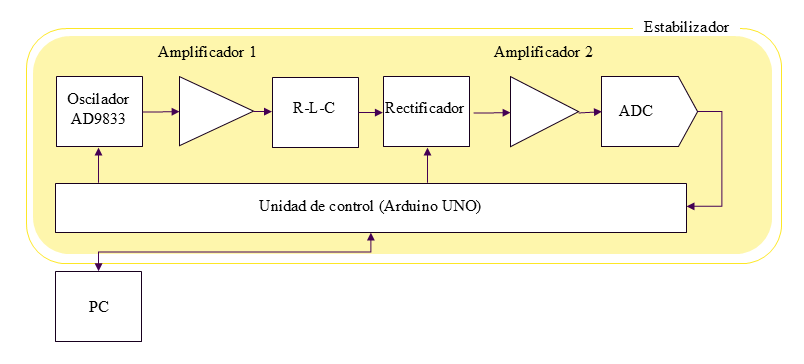
\includegraphics[width=1\linewidth]{SOLO-ESQUEMA.png}
\caption{Modulos del experimento.}
\label{fig:SOLO-ESQUEMA}
\end{center}
\end{figure} 

\subsection{modulo generador}

Se encarga de generar y suministrar la señal sinusoidal al cirucito resonante R-L-C.Se comopone de:
\begin{itemize}
  \item Oscilador AD9833: es un modulo electrónico comercial que permite generar señales muy estables y de INCLUIR CARACTERISTICAS DESTACABLE, REFERRENCIAR AL DATA SHEET
  \item Amplificador 1: Este se encarga de amplificar en voltaje y potencia la señal del generador, esto es necesario para poder excitar el ciruito resonante. INCLUIR LOS DOS CIRCUITOS QUE LO COMPONEN
\end{itemize} 

\subsection{Modulo de lectura}

\begin{itemize}
  \item Rectificador
  \item Amplificador 2 INCLUIR OPAM Y EL DE CANBERRA
  \item ADC INCLUIR SUS CARACTERISTICAS DESTACADAS QUE NOS HICIERON ELEGIRLO, Y REFERENCIAR AL  DATA SHEET
\end{itemize}

\subsection{modulo automatizacion}


\subsection{modulo estabilizador}



\section{Experimento RLC en Serie}
\subsection{procedimiento experimental}
\subsection{Resultados}

\section{Experimento RLC en paralelo}
\subsection{procedimiento experimental}
\subsection{Resultados}



Aquí va el diagrama del circuito y explicación de su funcionamiento
\begin{figure}[hbt]
\begin{center}
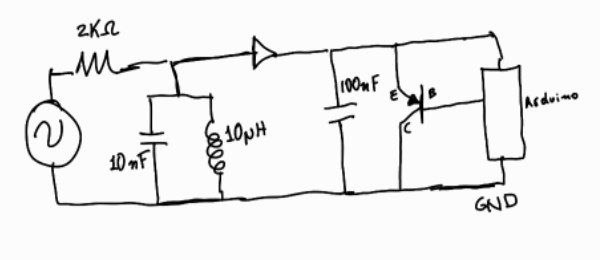
\includegraphics[scale=0.5]{circuitoDibujo.jpg}
\caption[circuito dibujado a mano alzada]{circuito dibujado a mano alzada}
\label{fig:figura1}
\end{center}
\end{figure} 

\begin{figure}[hbt]
\begin{center}
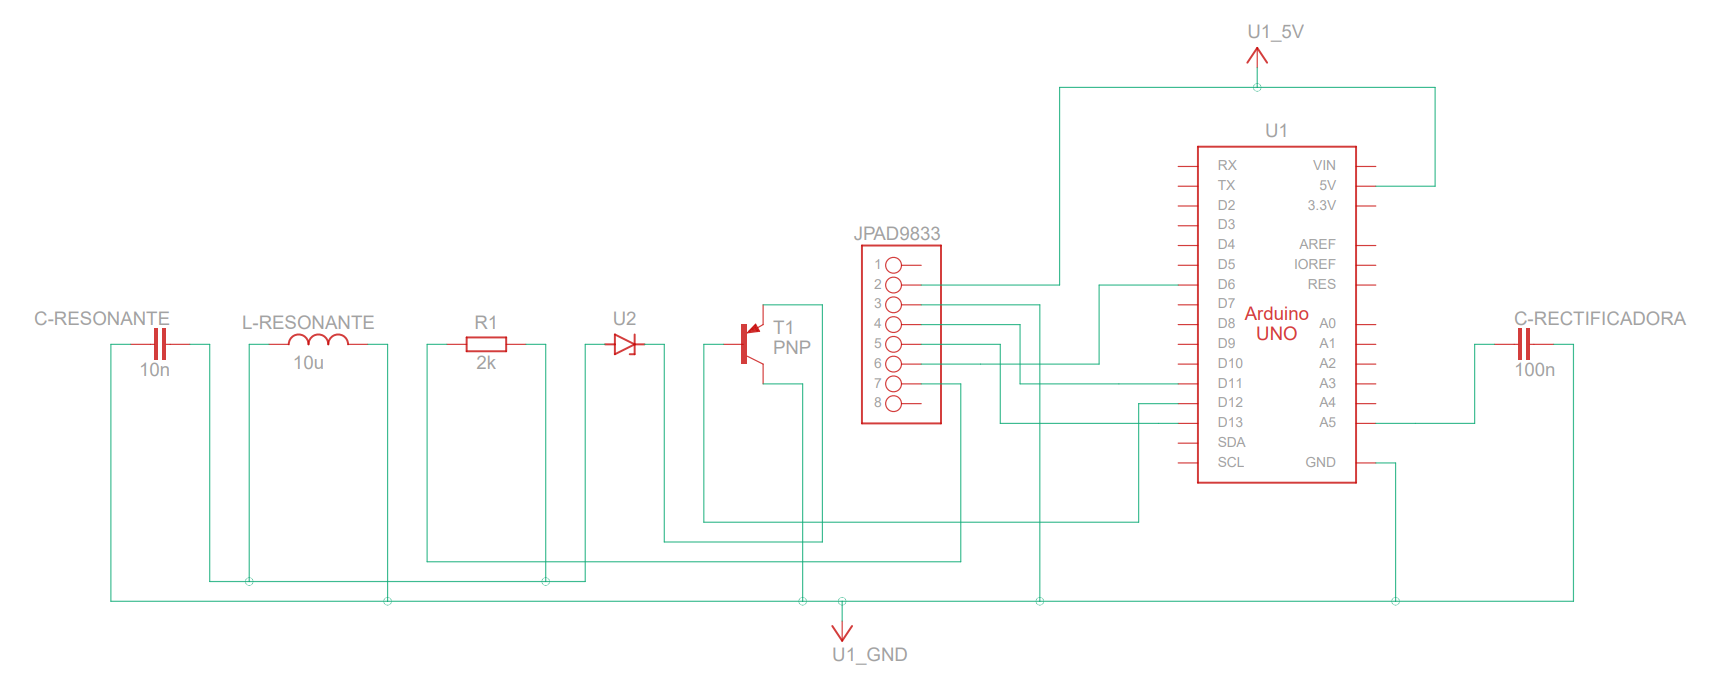
\includegraphics[scale=0.5]{CircuitoCAD.png}
\caption[circuito donde se explica claramente la conexión del arduino,]{circuito donde se explica claramente la conexión del arduino}
\label{fig:figura1}
\end{center}
\end{figure}

Los pines del generador de funciones AD9833 en el diagrama son 
  1-ref
  2-VCC
  3-GND
  4-DAT
  5-CLK
  6-FNC
  7-OUT


\section{Calculo de la precisión necesaria: Ajuste de la curva por ODR}


\section{Modificaciones propuestas} 




hablar sobre la propuesta de prof Julio Wlater
Hablar sobre cambiarse de arduino a red pitaya
